\section{Diseño y Arquitectura de Software}\label{cap:arquitectura}

La arquitectura original del sistema (Figura~\ref{fig:v4_2}) se mantiene como monolito modular y se amplía con los componentes de la propuesta Lush Beauty Smart. Este capítulo detalla sus principios, paquetes, modelo de datos, reglas de negocio, mecanismos de sincronización, seguridad y despliegue.

\subsection{Principios de arquitectura}

La solución adopta un monolito modular con capas de presentación, aplicación, dominio y persistencia. Los módulos se comunican mediante interfaces de servicio declaradas y no acceden directamente a tablas ajenas. La API constituye la autoridad sobre autenticación, validación, cálculos, auditoría y permisos. La IA consulta datos a través de servicios explícitos, y n8n recibe eventos derivados de operaciones confirmadas. La separación permite sustituir proveedores de IA o canales de notificación sin alterar la lógica contable.


\begin{figure}[H]
\caption{Arquitectura conceptual de Lush Beauty Smart}\label{fig:dss_2}
\centering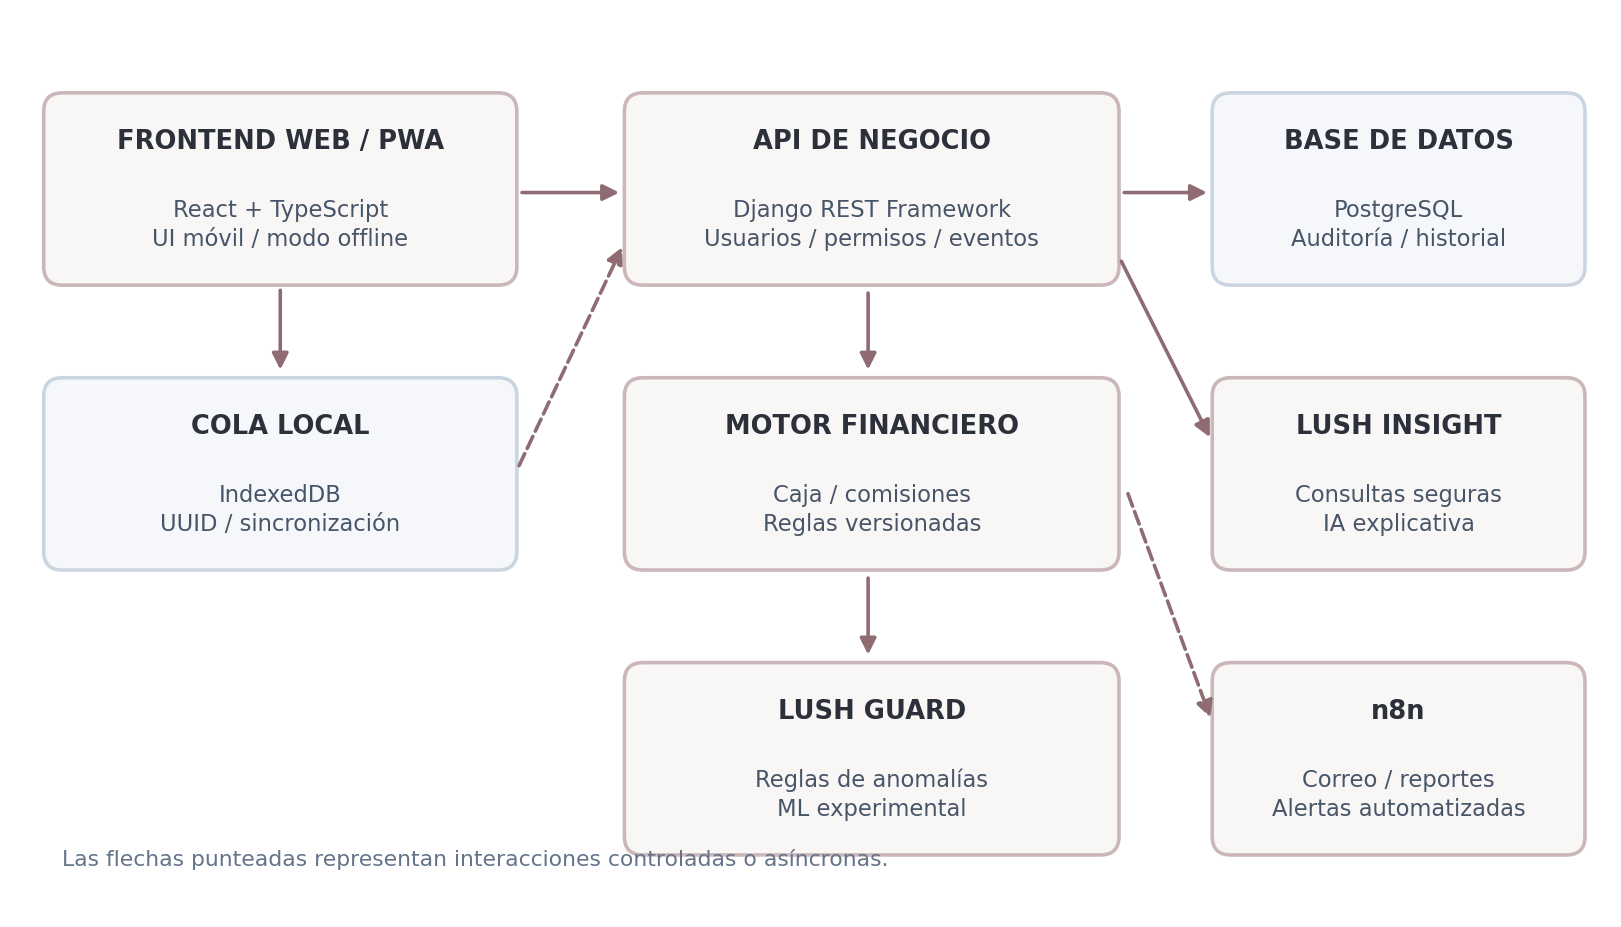
\includegraphics[width=0.9\linewidth]{img/fig_arquitectura_smart.png}
\end{figure}
\nota{Elaboración propia; no representa componentes desplegados en producción.}

\subsubsection{Incorporación de la capa de modelos DSS}

La arquitectura existente se mantiene como monolito modular. Se agregan paquetes independientes: decision\_scenarios para escenarios y sus parámetros, financial\_models para cálculo de contribución y proyección de caja, criteria\_evaluation para matriz y sensibilidad, recommendations para ensamblar explicaciones y decision\_outcomes para seguimiento. El API permite consultas de resultados, pero impide a un LLM invocar escrituras financieras directas. Los servicios DSS consumen datos agregados y snapshots versionados desde PostgreSQL; n8n solo reacciona a decisiones aprobadas.


\vspace{8pt}{\small\setstretch{1.0}
\begin{longtable}{>{\raggedright\arraybackslash}p{0.3333\dimexpr\linewidth-6\tabcolsep\relax}>{\raggedright\arraybackslash}p{0.3333\dimexpr\linewidth-6\tabcolsep\relax}>{\raggedright\arraybackslash}p{0.3333\dimexpr\linewidth-6\tabcolsep\relax}}
\caption{Paquetes adicionales del monolito para implementar el DSS}\label{tab:dss_16}\\
\toprule
\textbf{Servicio backend} & \textbf{Entradas} & \textbf{Salidas / controles} \\
\midrule\endfirsthead
\toprule
\textbf{Servicio backend} & \textbf{Entradas} & \textbf{Salidas / controles} \\
\midrule\endhead
\bottomrule\endfoot
\bottomrule\endlastfoot
financial\_models & Ventas, políticas, costos variables & Decimal; resultados con snapshot \\
decision\_scenarios & Parámetros no operativos de simulación & Resultados comparables y sin escrituras en ventas \\
criteria\_evaluation & Alternativas, escalas, pesos, restricciones & Puntuaciones, ranking y sensibilidad \\
recommendations & Resultados DSS ya calculados & Explicación trazable y estado de evidencia \\
decision\_outcomes & Aprobaciones y revisión posterior & Historial auditable y control por roles \\
\end{longtable}}

\subsection{Componentes y responsabilidades}

\vspace{8pt}{\small\setstretch{1.0}
\begin{longtable}{>{\raggedright\arraybackslash}p{0.3333\dimexpr\linewidth-6\tabcolsep\relax}>{\raggedright\arraybackslash}p{0.3333\dimexpr\linewidth-6\tabcolsep\relax}>{\raggedright\arraybackslash}p{0.3333\dimexpr\linewidth-6\tabcolsep\relax}}
\caption{Selección tecnológica propuesta; versiones concretas deben fijarse al iniciar el repositorio}\label{tab:dss_5}\\
\toprule
\textbf{Componente} & \textbf{Tecnología recomendada} & \textbf{Responsabilidad} \\
\midrule\endfirsthead
\toprule
\textbf{Componente} & \textbf{Tecnología recomendada} & \textbf{Responsabilidad} \\
\midrule\endhead
\bottomrule\endfoot
\bottomrule\endlastfoot
Cliente web/PWA & React, TypeScript & Registro, panel, consultas, estado offline \\
Caché y cola local & Service Worker, IndexedDB & Persistencia temporal y reintentos \\
API REST & Django, DRF & Identidad, permisos, validaciones, consultas \\
Dominio financiero & Python Decimal, servicios Django & Caja, comisiones, nómina, cierres \\
Base de datos & PostgreSQL & Entidades, constraints, snapshots, auditoría \\
Importador & openpyxl, RapidFuzz & Lectura XLSX, normalización y revisión \\
Lush Insight & LLM + herramientas de lectura & Explicaciones ancladas en consultas \\
Lush Guard & Reglas; scikit-learn opcional & Detección y clasificación de incidencias \\
Automatización & n8n, webhooks, eventos & Notificaciones y distribución controlada \\
Despliegue & Docker Compose, HTTPS & Reproducibilidad y entorno de feria \\
\end{longtable}}

\subsection{Modelo conceptual de datos}

Para mantener la trazabilidad se propone modelar cada transacción y cada regla en entidades explícitas. Las relaciones entre servicios, líneas de venta y pagos permitirán representar combos y pagos divididos sin fórmulas incrustadas en el frontend. Una liquidación aprobada conservará su versión y un detalle reproducible de cada concepto.


\vspace{8pt}{\small\setstretch{1.0}
\begin{longtable}{>{\raggedright\arraybackslash}p{0.3333\dimexpr\linewidth-6\tabcolsep\relax}>{\raggedright\arraybackslash}p{0.3333\dimexpr\linewidth-6\tabcolsep\relax}>{\raggedright\arraybackslash}p{0.3333\dimexpr\linewidth-6\tabcolsep\relax}}
\caption{Modelo conceptual inicial; los tipos de datos, índices y cardinalidades se especificarán en el diseño físico}\label{tab:dss_6}\\
\toprule
\textbf{Entidad} & \textbf{Campos fundamentales} & \textbf{Relación principal} \\
\midrule\endfirsthead
\toprule
\textbf{Entidad} & \textbf{Campos fundamentales} & \textbf{Relación principal} \\
\midrule\endhead
\bottomrule\endfoot
\bottomrule\endlastfoot
Salon & id, nombre, estado & Agrupa datos por tenant\_id \\
Usuario / Rol & id, salon\_id, rol, permisos & Acceso por operación \\
Especialista & id, salon\_id, usuario\_id & Realiza servicios \\
ServicioCatalogo & id, nombre, precio, vigencia & Identificado por líneas \\
Venta / LineaVenta & id, uuid\_cliente, importes, snapshots & Servicio y comisión aplicada \\
Pago & id, venta\_id, medio, monto & Distribución por método \\
ReglaComision & id, porcentaje, base, fecha\_inicio & Versión aplicada a líneas \\
Propina / Deduccion & id, especialista, importe, motivo & Integran liquidaciones \\
Liquidacion / Detalle & id, periodo, estado, total & Resumen firmado lógicamente \\
CierreCaja & id, fecha, diferencias, aprobador & Conciliación diaria \\
Auditoria / EventoOutbox & id, actor, antes/después, evento & Trazabilidad y automatización \\
Importacion / Incidencia & id, archivo, fila, estado & Correcciones supervisadas \\
\end{longtable}}

\subsection{Reglas de negocio críticas}

\begin{vinetas}
\item RN-01. Cada venta confirmada dispone de identificador único; los reintentos con la misma clave de idempotencia no crean duplicados.
\item RN-02. Una comisión usa porcentaje, base de cálculo y versión de regla vigentes al momento de la operación.
\item RN-03. Las sumas monetarias emplean Decimal y un criterio explícito de redondeo consistente con el acuerdo del salón.
\item RN-04. La suma de pagos confirmados debe coincidir con el importe cobrable, salvo estados parciales autorizados.
\item RN-05. Una liquidación aprobada no se sobrescribe; cualquier corrección genera un ajuste auditado.
\item RN-06. La especialista solo puede acceder a sus propios detalles y a datos operativos permitidos; la administradora autoriza políticas y cierres.
\item RN-07. Una incidencia detectada por IA o reglas no modifica por sí misma el registro financiero.
\item RN-08. Toda exportación o entrega de información salarial se limita al destinatario autorizado.
\end{vinetas}

\subsection{Sincronización offline e idempotencia}

Al registrar una venta, la PWA guarda una copia estructurada en IndexedDB y asigna un identificador idempotente. El proceso de sincronización transmite registros pendientes cuando hay red. El servidor verifica permisos, integridad, versiones del catálogo y presencia previa de la clave; confirma la transacción en un bloque atómico y devuelve su identificador. Si la red falla después de persistir la operación pero antes de recibir la respuesta, la repetición retorna el resultado original, evitando duplicidad.


Los conflictos se registran para resolución visible: por ejemplo, un precio que cambió mientras la venta estaba fuera de línea o un descuento no autorizado. El cliente no debe convertir un conflicto en una venta confirmada sin intervención. Las pruebas contemplan pérdida de red antes y después de enviar, dos intentos consecutivos y reinicio del teléfono.


\subsection{Diseño de Lush Insight}

El asistente opera con arquitectura de herramientas (tool calling) controladas. Una primera capa verifica el usuario y su tenant; una segunda clasifica la intención y valida fechas; una tercera invoca consultas de solo lectura definidas por contrato, que calculan métricas desde el dominio financiero; finalmente el modelo genera una redacción comprensible a partir de JSON de resultados. Se registran versión del prompt, herramienta consultada, filtros y referencia al reporte, evitando almacenar conversaciones con información sensible sin necesidad.


Ejemplo de contrato: obtener\_impacto\_descuentos(fecha\_inicio, fecha\_fin) devuelve monto\_bruto, descuentos, monto\_neto, comision\_lista, comision\_neto y politica\_vigente. La explicación puede comparar escenarios, pero nunca establecer un cambio de comisión ni ejecutar una transacción. Las respuestas sensibles requieren permisos específicos y se limitan a los períodos autorizados.


\subsection{Arquitectura de eventos y n8n}

Un patrón outbox transaccional permite insertar, junto con la operación aprobada, un evento pendiente de entrega. Un proceso posterior publica al webhook de n8n, que valida el mensaje y ejecuta acciones idempotentes. Si se produce un error temporal en el correo, el flujo puede reintentarse sin volver a contabilizar la nómina. El evento no contendrá más información de la necesaria; para documentos individuales se utilizarán enlaces de expiración corta con control de autorización.


\subsection{Seguridad, privacidad y observabilidad}

El despliegue debe utilizar HTTPS, autenticación robusta, roles, validación de entrada, control de acceso por salón en todas las consultas y registro de eventos críticos. El diseño plantea seguridad a nivel de fila (RLS); su implementación necesita pruebas que demuestren aislamiento efectivo, no solo la presencia de tenant\_id. La copia de seguridad deberá verificarse mediante restauración en un entorno de prueba. Los secretos de n8n y del proveedor de IA no se incluirán en el repositorio.


Los datos enviados a servicios de IA externos, si se utilizan, deben minimizarse y anonimizarse cuando sea posible. Se requiere autorización para procesar información del salón y evitar exponer nombres, teléfonos, salarios y detalles sensibles de clientes en logs o ejemplos de feria. En el entorno demostrativo se recomiendan registros sintéticos y nombres sustituidos por códigos.


\subsection{Estrategia de despliegue y mantenimiento}

Para la feria, Docker Compose puede levantar API, base de datos, frontend y n8n en un entorno reproducible. Se separan ambientes de desarrollo, demostración y piloto; no se reutiliza la base real en una demostración pública. Se documentan variables de entorno, copias de seguridad, migraciones, cuentas de prueba y un plan de funcionamiento sin servicio de IA: la caja, las comisiones y los reportes deben seguir operando cuando no esté disponible el asistente.

